\documentclass[../MATLAB_Primer.tex]{subfiles}
\begin{document}
It is important to understand and implement plotting features in MATLAB in order to better visualize problems and communicate results obtained from your models.  The plotting capabilities of MATLAB are in fact so useful that they were emulated in the popular Python package \texttt{matplotlib} which is the primary plotting library for most Python developers. The following section outlines plotting in 2-D and 3-D. 

\subsection{2-D Line Plots}
Most times you will be working with the 2-D line plot.  This type of plot is best suited for time-series and sampled data, as well as for visualizing scalar functions defined on real number line.  

\subsubsection{Basics}
In order to produce 2-D plots in MATLAB, we make use of the \texttt{plot} function.  This function generates highly customizable figure and axis objects with which our data can be visualized.

\begin{table}[H]
\caption{2D Plot Function}
    \begin{center}
        \begin{tabular}{| C{3cm} | m{12cm}|}
            \hline
            \textbf{MATLAB Syntax} & \textbf{Description}\\
            
            \hline
            \href{https://www.mathworks.com/help/matlab/ref/plot.html}{\color{blue}plot(X, Y)} & Generates a 2-D line plot for vector $Y$ versus $X$, where $X$ and $Y$ are of equal length.  \\
            \hline
        \end{tabular}
        \label{tab:2D_plotting}
    \end{center}
\end{table}

Example 1:\\

\textit{input:}
\begin{lstlisting}
x = linspace(-pi/2, pi/2, 100);

y1 = cos(x)  % generated from x => (x,y1) equal length
plot(x,y1);

hold on;    % hold on command allows multiple plots on same figure

y2 = 1 - (1/2).*x.^2 + (1/4).*x.^4;
plot(x,y2)

hold off;   % release the hold on command

\end{lstlisting}
\textit{output:}

\begin{figure}[H]
    \centering
    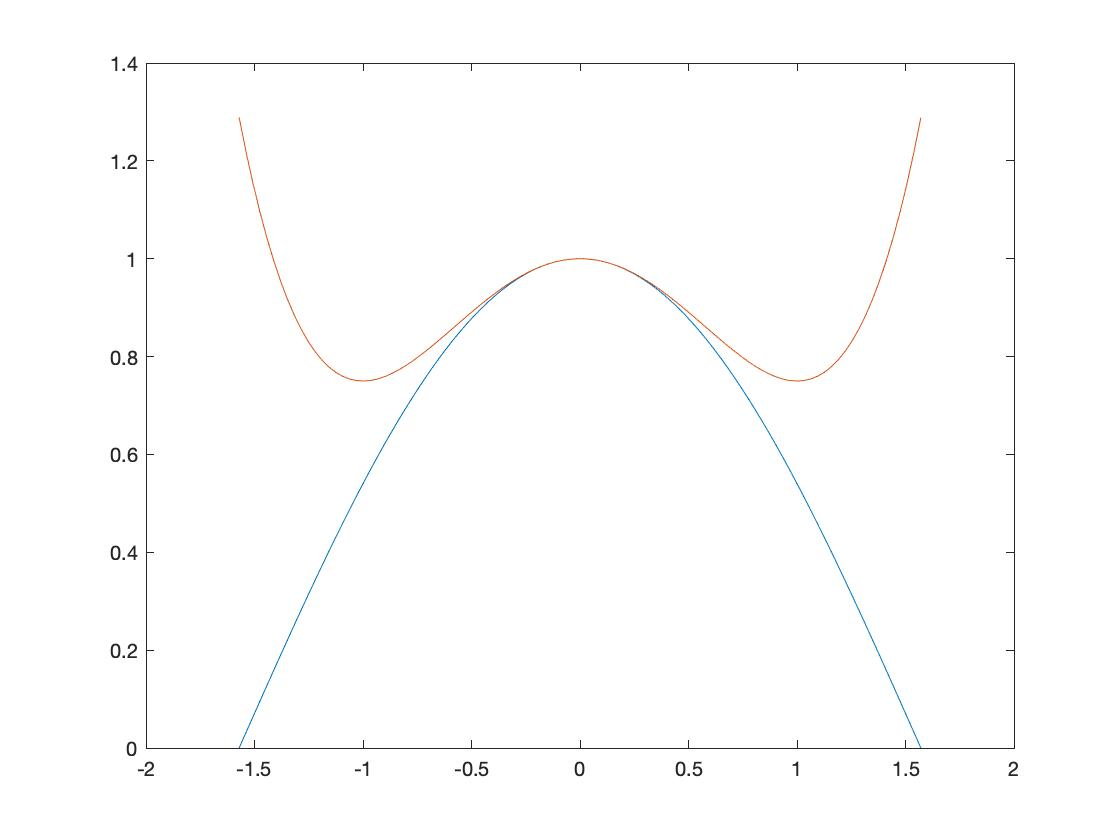
\includegraphics[width=350pt]{images/plotting_example1.jpg}
    \caption{Plotting cos(x) versus its fourth order Taylor approximation on [-$\frac{\pi}{2}$,$\frac{\pi}{2}$]}
    \label{fig:plotting_example1}
\end{figure}

Oftentimes we will wish to label the axes and plot itself.  This can be done through the addition of a few short commands.\\ 

Example 2:\\

\textit{input:}
\begin{lstlisting}
x = linspace(0, 10, 100);

y1 = x.^2;
y2 = x;

plot(x,y1);
hold on; 
plot(x,y2);

% plot a point 
plot([7], [30], 'ko');

% labelling
title('this is the title');
xlabel('this is our x-axis label');
ylabel('this is our y-axis label');


hold off;   % release the hold on command

\end{lstlisting}
\textit{output:}

\begin{figure}[H]
    \centering
    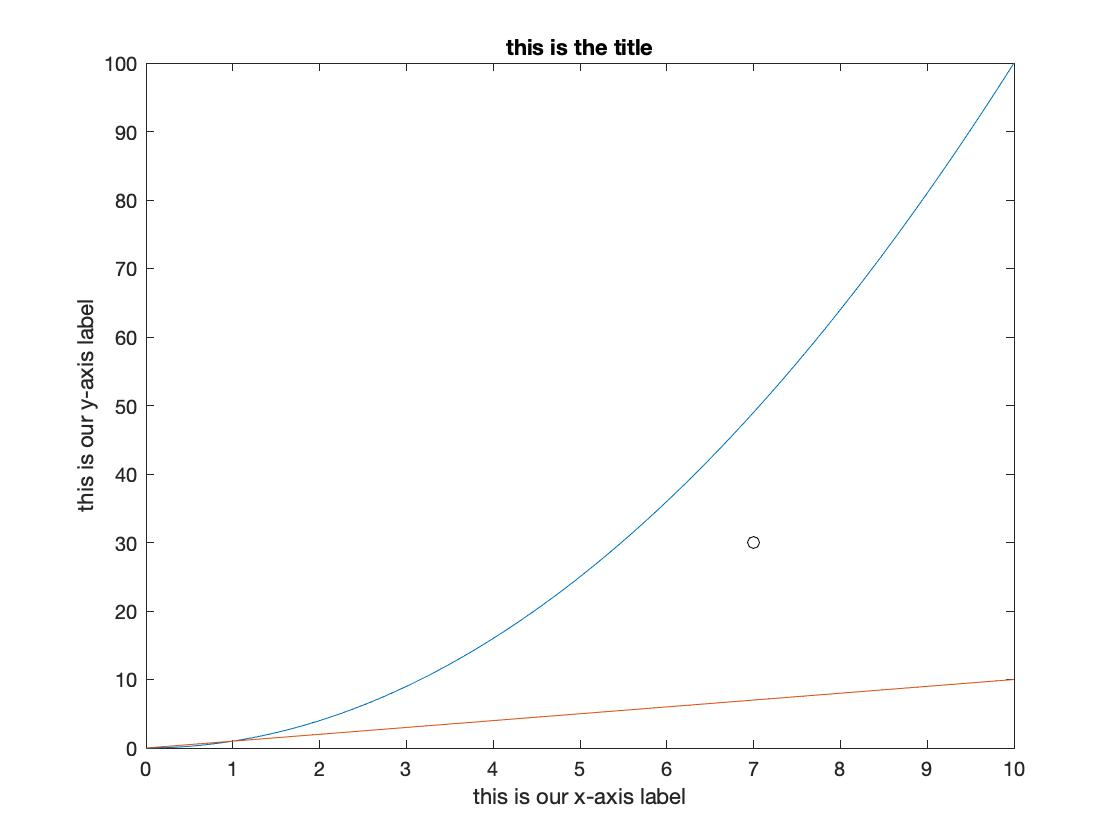
\includegraphics[width=350pt]{images/plotting_example2.jpg}
    \caption{Plot with axis labels and title}
    \label{fig:plotting_example2}
\end{figure}

\subsubsection{Customizing Plot Features}
Outside of the addition of labels and a title, we also have significant control over the line properties and figure elements.  Attributes such as line colour, line thickness, line style, and marker size are easily manipulated. Features such as legends and axis grids can also be implemented in a few lines of code. \\

In the following examples we will show some different methods for generating more customized plots.\\

Example 1:\\

\textit{input:}
\begin{lstlisting}
x = linspace(-5, 5, 100);
y1 = x.^2;
y2 = x.^3;

% customize lines using name-value pair arguments  
plot(x,y1, 'LineStyle', '--', 'color', 'b', 'LineWidth',0.5);
hold on 
plot(x,y2, 'color', 'r', 'LineWidth',2.5);

% label
xlabel('x');
ylabel('f(x)');

% we can change default axis limits 
xlim([-5 5]);
ylim([-5, 25]);

% add legend 
legend('x^2', 'x^3');
\end{lstlisting}
\textit{output:}

\begin{figure}[H]
    \centering
    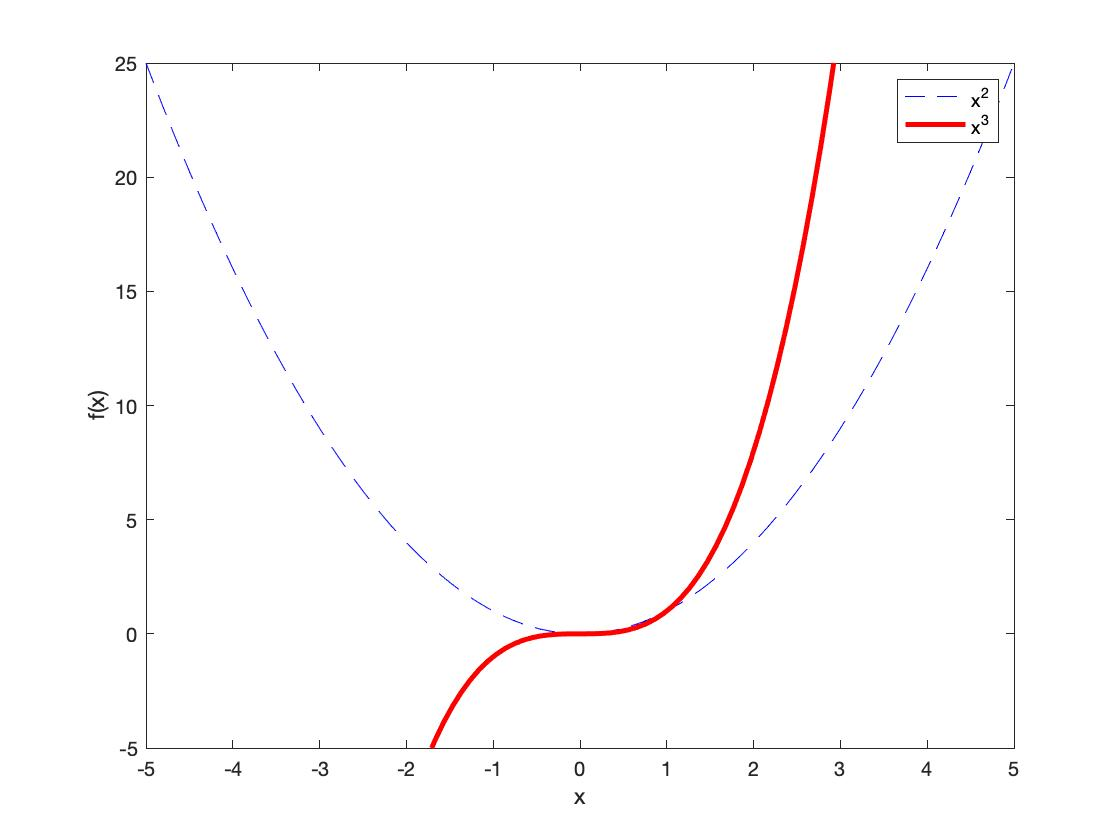
\includegraphics[width=350pt]{images/plotting_example3.jpg}
    \caption{Plotting with custom line properties}
    \label{fig:plotting_example3}
\end{figure}

Here we've modified line properties through the inclusion of ``Name-Value Pair Arguments" in the \texttt{plot} function call. For more information on the arguments available read the \href{https://www.mathworks.com/help/matlab/ref/plot.html#namevaluepairs}{\color{blue}official documentation}.\\

Lines objects can also be assigned to a variable and modified after the plot command.\\

Example 2:\\

\textit{input:}
\begin{lstlisting}
x = linspace(0, 20, 100);
y1 = log(x);
y2 = exp(-x);

% create line objects 
line1 = plot(x,y1);
hold on;
line2 = plot(x,y2);

% customize line object attributes
line1.LineWidth = 2;
line1.Color = "r";
line1.DisplayName = "log(x)";

line2.LineStyle = "-";
line2.Marker = "o";
line2.Color = "m";
line2.DisplayName = "e\^{}(-x)";    % LaTeX convention for e^(-x)

% labels
xlabel('x');
ylabel('f(x)');

% already named lines so we can call legend() as such
legend();

\end{lstlisting}
\textit{output:}

\begin{figure}[H]
    \centering
    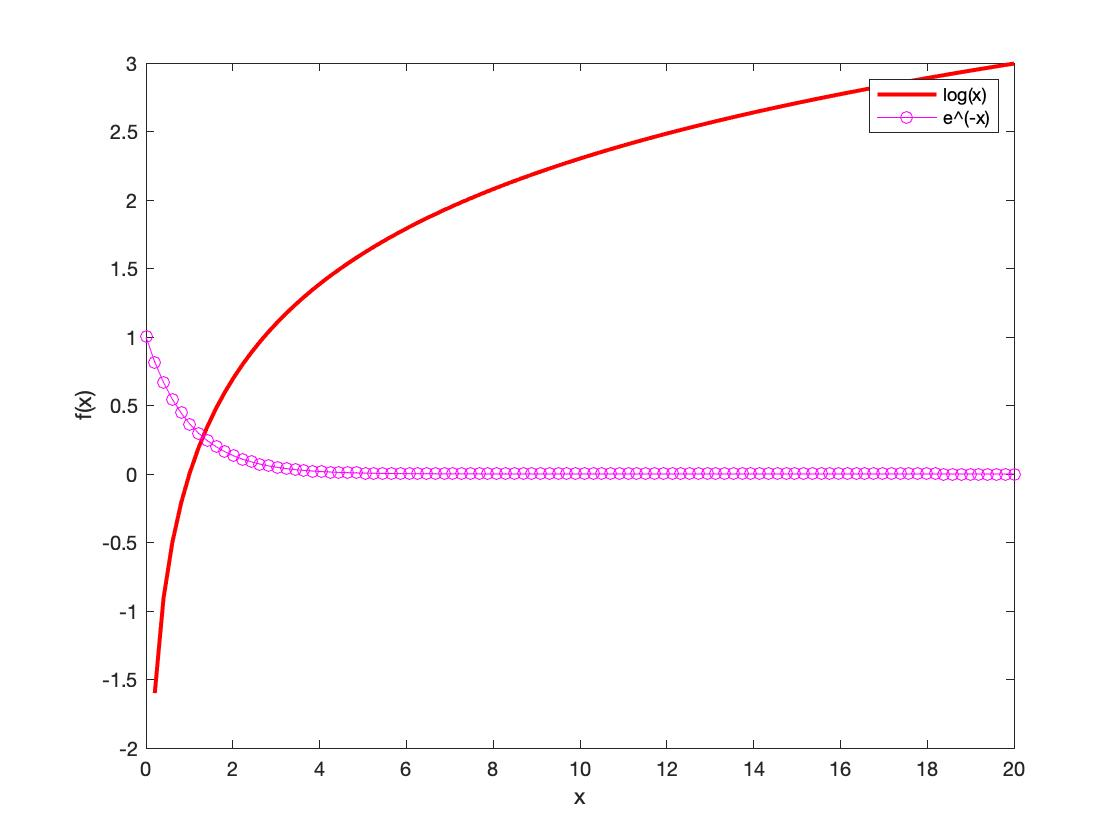
\includegraphics[width=350pt]{images/plotting_example4.jpg}
    \caption{Plotting with custom line properties}
    \label{fig:plotting_example4}
\end{figure}

\subsubsection{Subplots}
It can often be useful to visualize multiple plots in the same figure.  Implementing subplots in MATLAB can be accomplished through the use of the \texttt{subplot()} or \texttt{tiledlayout()} functions.\\

\begin{table}[H]
\caption{Subplot Function}
    \begin{center}
        \begin{tabular}{| C{3cm} | m{12cm}|}
            \hline
            \textbf{MATLAB Syntax} & \textbf{Description}\\
            
            \hline
            \href{https://www.mathworks.com/help/matlab/ref/subplot.html}{\color{blue}subplot(m,n,p)} & Divides the current figure into an $m$ $\times$ $n$ grid and plots in position $p$ \\
            \hline
            \href{https://www.mathworks.com/help/matlab/ref/subplot.html}{\color{blue}tiledlayout(m,n)} & Creates a tiled layout grid of size $m$ $\times$ $n$ \\
            \hline
        \end{tabular}
        \label{tab:subplotting}
    \end{center}
\end{table}

Review the following examples to better understand how each function works and to pick up on differences between the two functions.\\

Example 1:\\

\textit{input:}
\begin{lstlisting}
% plot using subplot 
x = linspace(-pi, pi);

subplot(2,1,1);     % 2 rows, 1 col, plot in position 1
y1 = cos(x);
plot(x,y1);

subplot(2,1,2);     % 2 rows, 1 col, plot in position 2
y2 = sin(x);
plot(x,y2);
\end{lstlisting}
\textit{output:}

\begin{figure}[H]
    \centering
    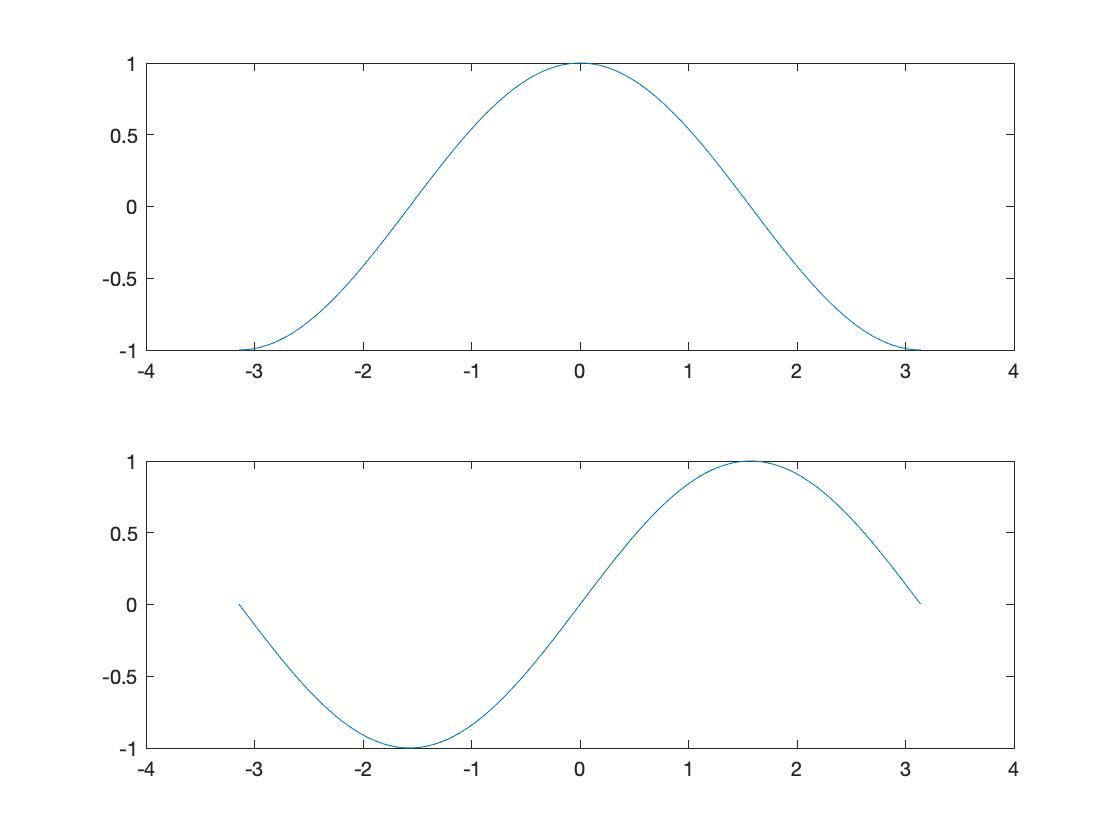
\includegraphics[width=350pt]{images/plotting_example5.jpg}
    \caption{Plotting cos(x) and sin(x) in subplot template}
    \label{fig:plotting_example5}
\end{figure}

Example 2:\\

\textit{input:}
\begin{lstlisting}
% plot using tiledlayout
x = linspace(-pi, pi);

tiledlayout(1,2);   % 1 row, 2 col

nexttile; % increments position in tiled layout
y1 = cos(x);
plot(x,y1);

nexttile;
y2 = sin(x);
plot(x,y2);

\end{lstlisting}
\textit{output:}

\begin{figure}[H]
    \centering
    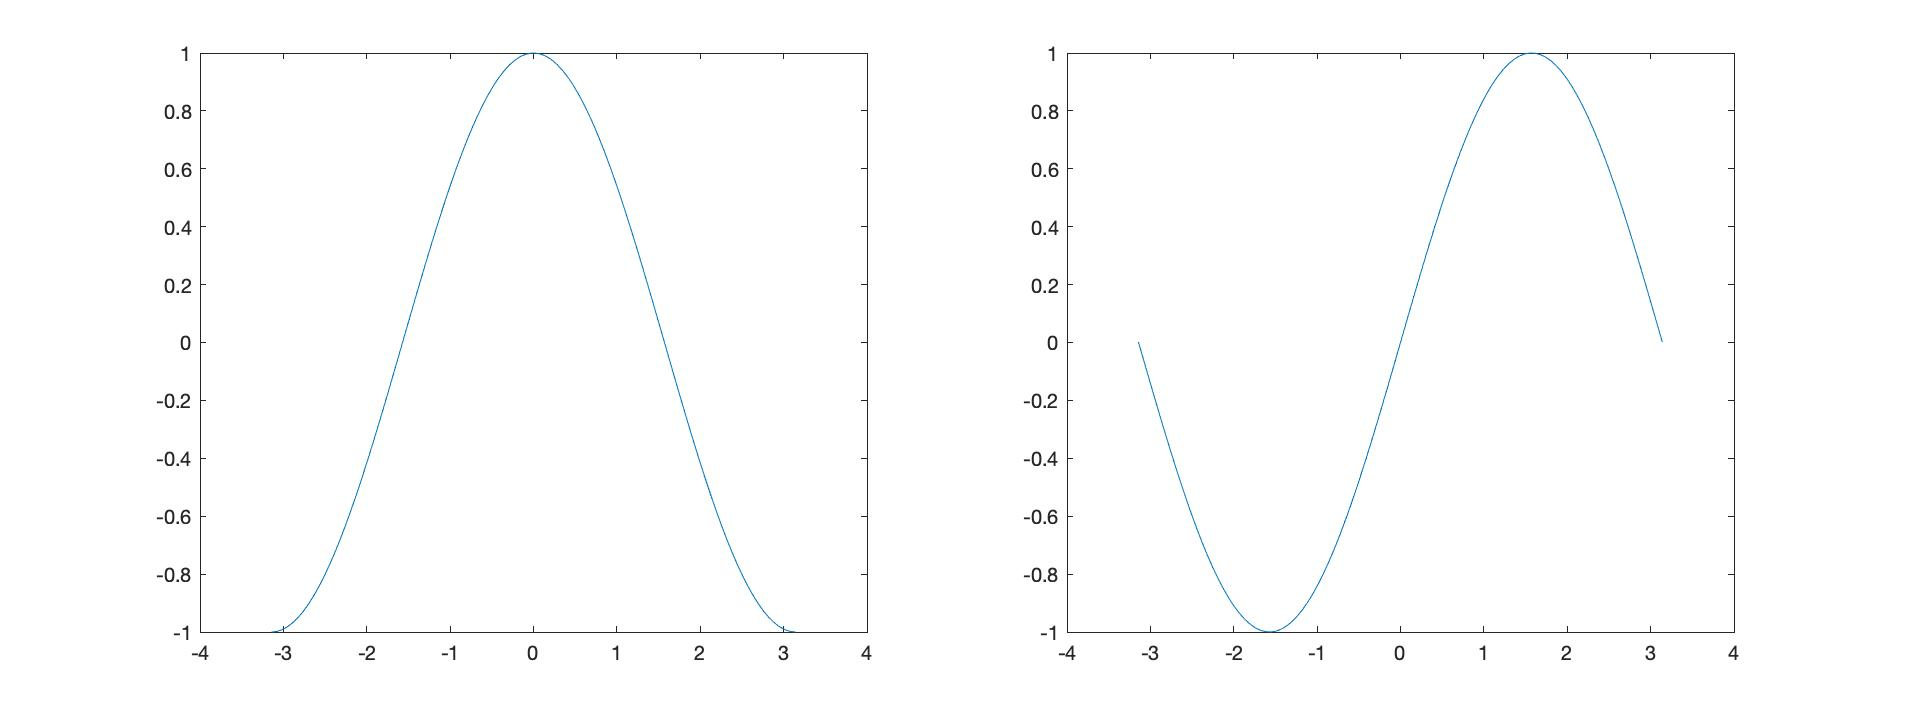
\includegraphics[width=350pt]{images/plotting_example5'.jpg}
    \caption{Plotting cos(x) and sin(x) in tiledlayout}
    \label{fig:plotting_example5'}
\end{figure}

Example 3:\\

\textit{input:}
\begin{lstlisting}
x = linspace(-1, 1);

tiledlayout(2,2);

nexttile;
y1 = x;
plot(x,y1, 'color', 'r', 'LineStyle', ':', 'LineWidth', 2);
title("first subplot");

nexttile;
y2 = x.^2;
plot(x,y2, 'color', 'b');
legend('line');
title("second subplot");

nexttile;
y3 = x.^3;
plot(x,y3, 'LineStyle', '-.', 'LineWidth', 1.5);
title("third subplot");

nexttile;
y4 = x.^4;
plot(x,y4);
grid on;
title("fourth subplot");
\end{lstlisting}
\textit{output:}

\begin{figure}[H]
    \centering
    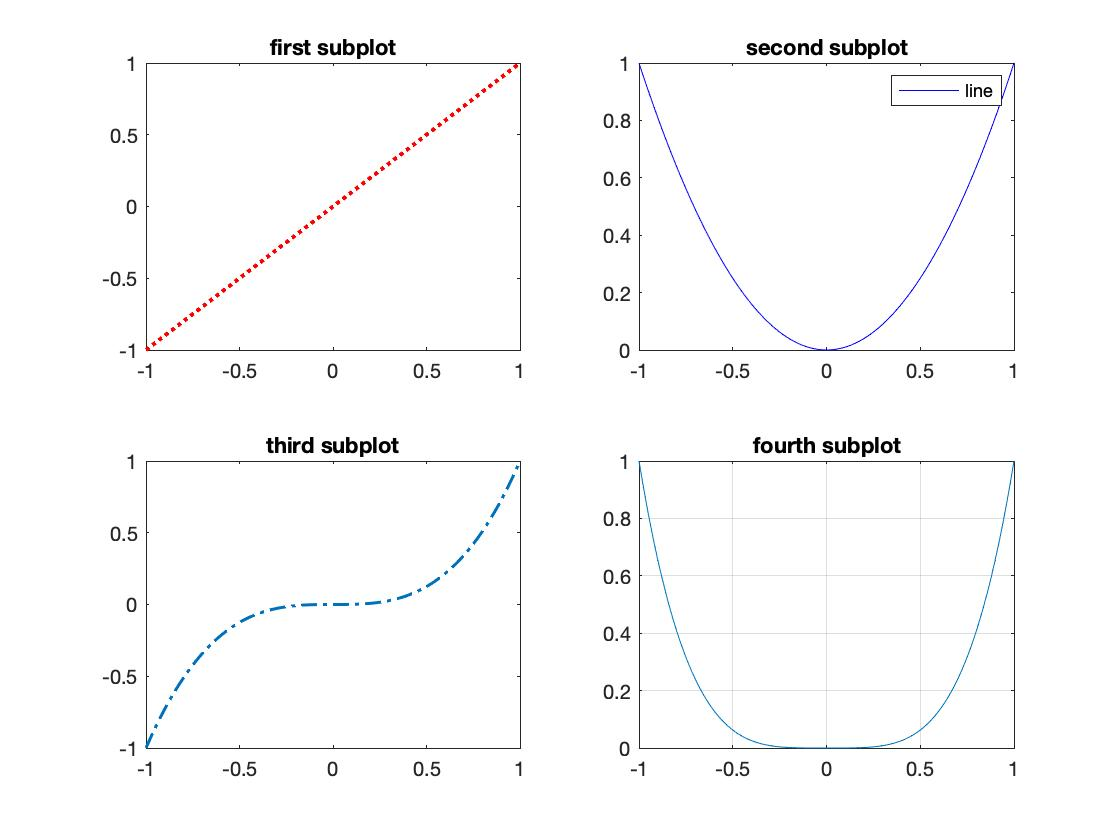
\includegraphics[width=350pt]{images/plotting_example6.jpg}
    \caption{Another subplot example, 2x2 grid}
    \label{fig:plotting_example6}
\end{figure}

The above example can be recreated using \texttt{subplot()} as follows:\\

Example 4:\\

\textit{input:}
\begin{lstlisting}
x = linspace(-1, 1);

subplot(2,2,1);     % 2 rows, 2 col, plot in position 1
y1 = x;
plot(x,y1, 'color', 'r', 'LineStyle', ':', 'LineWidth', 2);
title("first subplot");

subplot(2,2,2);     % plot in position 2
y2 = x.^2;
plot(x,y2, 'color', 'b');
legend('line');
title("second subplot");

subplot(2,2,3);     % plot in position 3
y3 = x.^3;
plot(x,y3, 'LineStyle', '-.', 'LineWidth', 1.5);
title("third subplot");

subplot(2,2,4);     % plot in position 4
y4 = x.^4;
plot(x,y4);
grid on;
title("fourth subplot");
\end{lstlisting}

Though both plotting functions accomplish the task of generating subplots, it is recommended to use \texttt{tiledlayout()} since it produces more readable and straightforward code.

\subsubsection{Graph Objects}
Graph objects represent undirected graphs, which is a set of nodes with edges connecting the nodes together. The \texttt{graph} function takes in the square and symmetric adjacency matrix \texttt{A} and returns the graph object \texttt{G}. Additionally, graph objects have two properties, \texttt{Edges} and \texttt{Nodes}. The \texttt{Edges} property holds data regarding the edges of the graph such as the end nodes connected by edges and the weight of the edges. The \texttt{Nodes} property holds data regarding the nodes of the graph such as the names of the nodes. Furthermore, the graph can be plotted using the \texttt{plot} function.
\\ \\
Example 1:
\\ \\
\textit{input:}
\begin{lstlisting}
% suppose there are 5 agents in R^2, each with a communication radius of 5
agentPos = [3 4;
            6 7;
            1 5;
            9 3;
            2 4;];
r = 5;

% create the distance matrix D
D = pdist(agentPos);
D = squareform(D);

% create the adjacency matrix A
A = D<=r;
A = A - eye(size(A,1));

% crete and plot the graph G
G = graph(A);
plot(G)
\end{lstlisting}
\textit{output:}
\begin{center}
    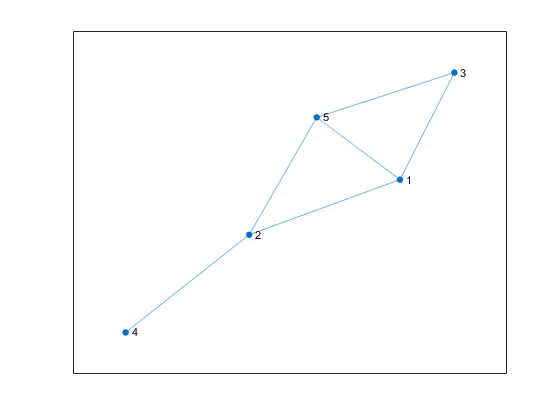
\includegraphics[width=250pt]{images/graph_output.png}
\end{center}

Example 2:
\\ \\
\textit{input:}
\begin{lstlisting}
% add property 'Names' to the graph nodes
names = {'Agent 1'; 
         'Agent 2'; 
         'Agent 3'; 
         'Agent 4'; 
         'Agent 5'};
         
G.Nodes.Names = names;
nodes = G.Nodes

\end{lstlisting}
\textit{output:}

\begin{center}
   nodes = 5x1 table 
\end{center}

\begin{table}[H]

    \begin{center}
        \begin{tabular}{|l|l|}
            \hline
             & \textbf{Names}\\
            
            \hline
            \textbf{1} & 'Agent 1' \\
            \hline
            \textbf{2} & 'Agent 2' \\
            \hline
            \textbf{3} & 'Agent 3' \\
            \hline
            \textbf{4} & 'Agent 4' \\
            \hline
            \textbf{5} & 'Agent 5' \\
            \hline
        \end{tabular}
    \end{center}
\end{table}

Example 3:
\\ \\
\textit{input:}
\begin{lstlisting}
edges = G.Edges

\end{lstlisting}
\textit{output:}

\begin{center}
   edges = 6x2 table 
\end{center}

\begin{table}[H]

    \begin{center}
        \begin{tabular}{|l|l|l|l|}
            \hline
            
             & \multicolumn{2}{l|}{\textbf{EndNodes}} & \textbf{Weight}\\
            
            \hline
            \textbf{1} & 1 & 2 & 1 \\
            \hline
            \textbf{2} & 1 & 3 & 1 \\
            \hline
            \textbf{3} & 1 & 5 & 1 \\
            \hline
            \textbf{4} & 2 & 4 & 1 \\
            \hline
            \textbf{5} & 2 & 5 & 1 \\
            \hline
            \textbf{6} & 3 & 5 & 1 \\
            \hline
        \end{tabular}
    \end{center}
\end{table}

\subsection{Plotting in 3-D}
Generating 3-D plots in MATLAB is syntactically similar to how we produced 2-D plots in the section above.  The only difference is that we have a bit more information to keep track of. 
\subsubsection{Meshgrid}
\texttt{meshgrid} is essentially the 3-D analogue of the \texttt{linspace} function in 2-D.  This function allows us to easily generate a grid upon which we can evaluate scalar functions.  This will make more sense as we observe the examples below. 

\begin{table}[H]
\caption{Mesh Generation}
    \begin{center}
        \begin{tabular}{| C{3cm} | m{12cm}|}
            \hline
            \textbf{MATLAB Syntax} & \textbf{Description}\\
            
            \hline
            \href{https://www.mathworks.com/help/matlab/ref/meshgrid.html}{\color{blue}meshgrid(X, Y)} & Generates a 2-D grid from vectors $X$ and $Y$ \\
            \hline
        \end{tabular}
        \label{tab:mesh}
    \end{center}
\end{table}

Example 1:\\

\textit{input:}
\begin{lstlisting}
x = 1:3;    % vector of unit-spaced points from 1 to 3
y = 1:3;

[X, Y] = meshgrid(x,y); % returns matrices X and Y

disp(X)
disp(Y)
\end{lstlisting}
\textit{output:}
\begin{center}
    X = 
    $\begin{bmatrix}
    1 & 2 & 3\\
    1 & 2 & 3\\
    1 & 2 & 3\\
    \end{bmatrix}$,\quad 
    Y = 
    $\begin{bmatrix}
    1 & 1 & 1\\
    2 & 2 & 2\\
    3 & 3 & 3\\
    \end{bmatrix}$
\end{center}

By superimposing the returned matrices from the \texttt{meshgrid} call, we can better understand what we are looking at. Indeed, $X$ and $Y$ are nothing other than matrices storing the x and y coordinates of a grid generated by the input arguments.\\
\begin{center}
    $\begin{bmatrix}
    (1,1) & (2,1) & (3,1)\\
    (2,1) & (2,2) & (3,2)\\
    (3,1) & (3,2) & (3,3)\\
    \end{bmatrix}$
\end{center}
In other words, \texttt{meshgrid} allows us to re-create a subset of the Cartesian plane numerically.\\

Example 2:\\

\textit{input:}
\begin{lstlisting}
x = linspace(-10,10);
y = linspace(-10,10);

[X, Y] = meshgrid(x,y);

% define a surface over the grid 
Z = X.^2 + Y.^2;

% plot 
surf(X,Y,Z)
\end{lstlisting}
\textit{output:}
\begin{figure}[H]
    \centering
    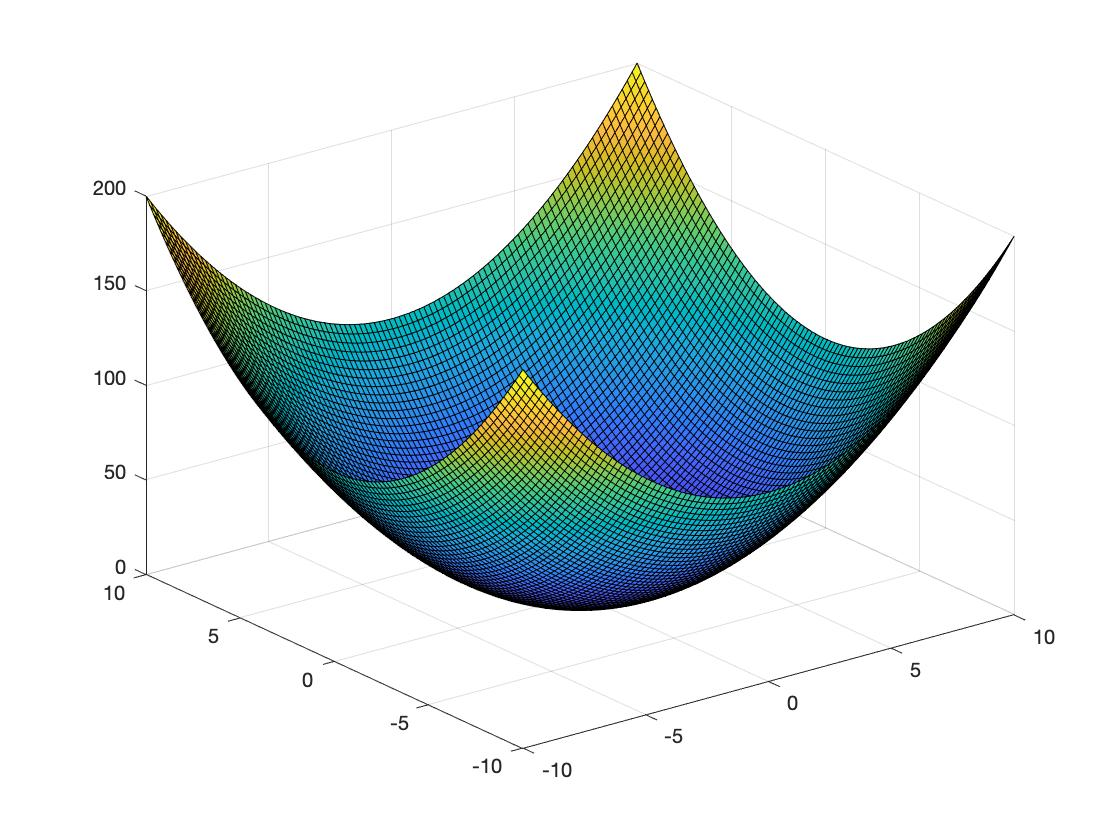
\includegraphics[width=350pt]{images/plotting_example7.jpg}
    \caption{Plotting $z^{2} - x^{2} - y^{2} = 0$}
    \label{fig:plotting_example7}
\end{figure}

\subsubsection{Plotting}
In order to generate 3-D plots in MATLAB we make use of the functions listed in the table below. 

\begin{table}[H]
\caption{3-D Plotting Functions}
    \begin{center}
        \begin{tabular}{| C{3cm} | m{12cm}|}
            \hline
            \textbf{MATLAB Syntax} & \textbf{Description}\\
            
            \hline
            \href{https://www.mathworks.com/help/matlab/ref/surf.html}{\color{blue}surf(X, Y, Z)} & Produces the surface $Z$ over meshgrid $(X,Y)$ \\
            \hline
            \href{https://www.mathworks.com/help/matlab/ref/plot3.html}{\color{blue}plot3(X, Y, Z)} & Produces a scatter plot of points in matrix $Z$ over meshgrid $(X,Y)$ \\
            \hline
        \end{tabular}
        \label{tab:3D_plotting}
    \end{center}
\end{table}



\end{document}